\documentclass[12pt,ngerman,]{book}
\usepackage{lmodern}
\usepackage{amssymb,amsmath}
\usepackage{ifxetex,ifluatex}
\usepackage{fixltx2e} % provides \textsubscript
\ifnum 0\ifxetex 1\fi\ifluatex 1\fi=0 % if pdftex
  \usepackage[T1]{fontenc}
  \usepackage[utf8]{inputenc}
\else % if luatex or xelatex
  \ifxetex
    \usepackage{mathspec}
  \else
    \usepackage{fontspec}
  \fi
  \defaultfontfeatures{Ligatures=TeX,Scale=MatchLowercase}
\fi
% use upquote if available, for straight quotes in verbatim environments
\IfFileExists{upquote.sty}{\usepackage{upquote}}{}
% use microtype if available
\IfFileExists{microtype.sty}{%
\usepackage{microtype}
\UseMicrotypeSet[protrusion]{basicmath} % disable protrusion for tt fonts
}{}
\usepackage[margin=1in]{geometry}
\usepackage{hyperref}
\PassOptionsToPackage{usenames,dvipsnames}{color} % color is loaded by hyperref
\hypersetup{unicode=true,
            pdftitle={Praxis der Datenanalyse ENTWURF},
            pdfauthor={Sebastian Sauer. Mit Beiträgen von Oliver Gansser, Matthias Gehrke und Karsten Lübke},
            colorlinks=true,
            linkcolor=Maroon,
            citecolor=Blue,
            urlcolor=Blue,
            breaklinks=true}
\urlstyle{same}  % don't use monospace font for urls
\ifnum 0\ifxetex 1\fi\ifluatex 1\fi=0 % if pdftex
  \usepackage[shorthands=off,main=ngerman]{babel}
\else
  \usepackage{polyglossia}
  \setmainlanguage[]{german}
\fi
\usepackage{color}
\usepackage{fancyvrb}
\newcommand{\VerbBar}{|}
\newcommand{\VERB}{\Verb[commandchars=\\\{\}]}
\DefineVerbatimEnvironment{Highlighting}{Verbatim}{commandchars=\\\{\}}
% Add ',fontsize=\small' for more characters per line
\usepackage{framed}
\definecolor{shadecolor}{RGB}{248,248,248}
\newenvironment{Shaded}{\begin{snugshade}}{\end{snugshade}}
\newcommand{\KeywordTok}[1]{\textcolor[rgb]{0.13,0.29,0.53}{\textbf{{#1}}}}
\newcommand{\DataTypeTok}[1]{\textcolor[rgb]{0.13,0.29,0.53}{{#1}}}
\newcommand{\DecValTok}[1]{\textcolor[rgb]{0.00,0.00,0.81}{{#1}}}
\newcommand{\BaseNTok}[1]{\textcolor[rgb]{0.00,0.00,0.81}{{#1}}}
\newcommand{\FloatTok}[1]{\textcolor[rgb]{0.00,0.00,0.81}{{#1}}}
\newcommand{\ConstantTok}[1]{\textcolor[rgb]{0.00,0.00,0.00}{{#1}}}
\newcommand{\CharTok}[1]{\textcolor[rgb]{0.31,0.60,0.02}{{#1}}}
\newcommand{\SpecialCharTok}[1]{\textcolor[rgb]{0.00,0.00,0.00}{{#1}}}
\newcommand{\StringTok}[1]{\textcolor[rgb]{0.31,0.60,0.02}{{#1}}}
\newcommand{\VerbatimStringTok}[1]{\textcolor[rgb]{0.31,0.60,0.02}{{#1}}}
\newcommand{\SpecialStringTok}[1]{\textcolor[rgb]{0.31,0.60,0.02}{{#1}}}
\newcommand{\ImportTok}[1]{{#1}}
\newcommand{\CommentTok}[1]{\textcolor[rgb]{0.56,0.35,0.01}{\textit{{#1}}}}
\newcommand{\DocumentationTok}[1]{\textcolor[rgb]{0.56,0.35,0.01}{\textbf{\textit{{#1}}}}}
\newcommand{\AnnotationTok}[1]{\textcolor[rgb]{0.56,0.35,0.01}{\textbf{\textit{{#1}}}}}
\newcommand{\CommentVarTok}[1]{\textcolor[rgb]{0.56,0.35,0.01}{\textbf{\textit{{#1}}}}}
\newcommand{\OtherTok}[1]{\textcolor[rgb]{0.56,0.35,0.01}{{#1}}}
\newcommand{\FunctionTok}[1]{\textcolor[rgb]{0.00,0.00,0.00}{{#1}}}
\newcommand{\VariableTok}[1]{\textcolor[rgb]{0.00,0.00,0.00}{{#1}}}
\newcommand{\ControlFlowTok}[1]{\textcolor[rgb]{0.13,0.29,0.53}{\textbf{{#1}}}}
\newcommand{\OperatorTok}[1]{\textcolor[rgb]{0.81,0.36,0.00}{\textbf{{#1}}}}
\newcommand{\BuiltInTok}[1]{{#1}}
\newcommand{\ExtensionTok}[1]{{#1}}
\newcommand{\PreprocessorTok}[1]{\textcolor[rgb]{0.56,0.35,0.01}{\textit{{#1}}}}
\newcommand{\AttributeTok}[1]{\textcolor[rgb]{0.77,0.63,0.00}{{#1}}}
\newcommand{\RegionMarkerTok}[1]{{#1}}
\newcommand{\InformationTok}[1]{\textcolor[rgb]{0.56,0.35,0.01}{\textbf{\textit{{#1}}}}}
\newcommand{\WarningTok}[1]{\textcolor[rgb]{0.56,0.35,0.01}{\textbf{\textit{{#1}}}}}
\newcommand{\AlertTok}[1]{\textcolor[rgb]{0.94,0.16,0.16}{{#1}}}
\newcommand{\ErrorTok}[1]{\textcolor[rgb]{0.64,0.00,0.00}{\textbf{{#1}}}}
\newcommand{\NormalTok}[1]{{#1}}
\usepackage{longtable,booktabs}
\usepackage{graphicx,grffile}
\makeatletter
\def\maxwidth{\ifdim\Gin@nat@width>\linewidth\linewidth\else\Gin@nat@width\fi}
\def\maxheight{\ifdim\Gin@nat@height>\textheight\textheight\else\Gin@nat@height\fi}
\makeatother
% Scale images if necessary, so that they will not overflow the page
% margins by default, and it is still possible to overwrite the defaults
% using explicit options in \includegraphics[width, height, ...]{}
\setkeys{Gin}{width=\maxwidth,height=\maxheight,keepaspectratio}
\IfFileExists{parskip.sty}{%
\usepackage{parskip}
}{% else
\setlength{\parindent}{0pt}
\setlength{\parskip}{6pt plus 2pt minus 1pt}
}
\setlength{\emergencystretch}{3em}  % prevent overfull lines
\providecommand{\tightlist}{%
  \setlength{\itemsep}{0pt}\setlength{\parskip}{0pt}}
\setcounter{secnumdepth}{5}
% Redefines (sub)paragraphs to behave more like sections
\ifx\paragraph\undefined\else
\let\oldparagraph\paragraph
\renewcommand{\paragraph}[1]{\oldparagraph{#1}\mbox{}}
\fi
\ifx\subparagraph\undefined\else
\let\oldsubparagraph\subparagraph
\renewcommand{\subparagraph}[1]{\oldsubparagraph{#1}\mbox{}}
\fi

%%% Use protect on footnotes to avoid problems with footnotes in titles
\let\rmarkdownfootnote\footnote%
\def\footnote{\protect\rmarkdownfootnote}

%%% Change title format to be more compact
\usepackage{titling}

% Create subtitle command for use in maketitle
\newcommand{\subtitle}[1]{
  \posttitle{
    \begin{center}\large#1\end{center}
    }
}

\setlength{\droptitle}{-2em}
  \title{Praxis der Datenanalyse ENTWURF}
  \pretitle{\vspace{\droptitle}\centering\huge}
  \posttitle{\par}
\subtitle{Skript zum Modul}
  \author{Sebastian Sauer. Mit Beiträgen von Oliver Gansser, Matthias Gehrke und
Karsten Lübke}
  \preauthor{\centering\large\emph}
  \postauthor{\par}
  \predate{\centering\large\emph}
  \postdate{\par}
  \date{07 June, 2017}

\usepackage{booktabs}
\usepackage{longtable}
\usepackage[bf,singlelinecheck=off]{caption}

%ses:
\pagestyle{headings}

%\setmainfont[UprightFeatures={SmallCapsFont=AlegreyaSC-Regular}]{Alegreya}

\usepackage{framed,color}
\definecolor{shadecolor}{RGB}{248,248,248}

\renewcommand{\textfraction}{0.05}
\renewcommand{\topfraction}{0.8}
\renewcommand{\bottomfraction}{0.8}
\renewcommand{\floatpagefraction}{0.75}

%\renewenvironment{quote}{\begin{VF}}{\end{VF}}
\let\oldhref\href
\renewcommand{\href}[2]{#2\footnote{\url{#1}}}

\ifxetex
  \usepackage{letltxmacro}
  \setlength{\XeTeXLinkMargin}{1pt}
  \LetLtxMacro\SavedIncludeGraphics\includegraphics
  \def\includegraphics#1#{% #1 catches optional stuff (star/opt. arg.)
    \IncludeGraphicsAux{#1}%
  }%
  \newcommand*{\IncludeGraphicsAux}[2]{%
    \XeTeXLinkBox{%
      \SavedIncludeGraphics#1{#2}%
    }%
  }%
\fi

% Hier müsste noch das Chapter mit rein! Sonst gibt es Das nicht in der Ausgabe!
% Daher habe ich das auskommentiert! (NM)
%\renewcommand{\thesection}{\arabic{section}}  % ses


\makeatletter
\newenvironment{kframe}{%
\medskip{}
\setlength{\fboxsep}{.8em}
 \def\at@end@of@kframe{}%
 \ifinner\ifhmode%
  \def\at@end@of@kframe{\end{minipage}}%
  \begin{minipage}{\columnwidth}%
 \fi\fi%
 \def\FrameCommand##1{\hskip\@totalleftmargin \hskip-\fboxsep
 \colorbox{shadecolor}{##1}\hskip-\fboxsep
     % There is no \\@totalrightmargin, so:
     \hskip-\linewidth \hskip-\@totalleftmargin \hskip\columnwidth}%
 \MakeFramed {\advance\hsize-\width
   \@totalleftmargin\z@ \linewidth\hsize
   \@setminipage}}%
 {\par\unskip\endMakeFramed%
 \at@end@of@kframe}
\makeatother

\renewenvironment{Shaded}{\begin{kframe}}{\end{kframe}}

\newenvironment{rmdblock}[1]
  {
  \begin{itemize}
  \renewcommand{\labelitemi}{
    \raisebox{-.7\height}[0pt][0pt]{
      {\setkeys{Gin}{width=3em,keepaspectratio}\includegraphics{images/#1}}
    }
  }
  \setlength{\fboxsep}{1em}
  \begin{kframe}
  \item
  }
  {
  \end{kframe}
  \end{itemize}
  }
\newenvironment{rmdnote}
  {\begin{rmdblock}{note}}
  {\end{rmdblock}}
\newenvironment{rmdcaution}
  {\begin{rmdblock}{caution}}
  {\end{rmdblock}}
\newenvironment{rmdimportant}
  {\begin{rmdblock}{important}}
  {\end{rmdblock}}
\newenvironment{rmdtip}
  {\begin{rmdblock}{tip}}
  {\end{rmdblock}}
\newenvironment{rmdwarning}
  {\begin{rmdblock}{warning}}
  {\end{rmdblock}}
\newenvironment{rmdpseudocode}
  {\begin{rmdblock}{pseudocode}}
  {\end{rmdblock}}
\newenvironment{rmdexercises}
  {\begin{rmdblock}{exercises}}
  {\end{rmdblock}}
\newenvironment{rmdlove}
  {\begin{rmdblock}{love}}
  {\end{rmdblock}}

\usepackage{makeidx}  % ses
\makeindex  % ses

\urlstyle{tt}

\usepackage{amsthm}
\makeatletter
\def\thm@space@setup{%
  \thm@preskip=8pt plus 2pt minus 4pt
  \thm@postskip=\thm@preskip
}


%NM:
\def\@makechapterhead#1{%
  \vspace*{50\p@}%
  {\parindent \z@ \raggedright \normalfont
  \ifnum \c@secnumdepth >\m@ne
    \if@mainmatter
        \huge\scshape\bfseries\scshape \@chapapp\space \thechapter
        \par\nobreak
        \vskip 20\p@
    \fi
  \fi
  \interlinepenalty\@M
  \Huge \scshape\bfseries\scshape #1\par\nobreak
  \vskip 40\p@
}}

\makeatother


% NM: Zu einem frontmatter gehört auch ein mainmatter, appendix und backmatter! ;-) - Habe ich daher mal eingefügt!
\frontmatter

\let\BeginKnitrBlock\begin \let\EndKnitrBlock\end
\begin{document}
\maketitle

{
\hypersetup{linkcolor=black}
\setcounter{tocdepth}{2}
\tableofcontents
}
\listoftables
\listoffigures
\chapter*{Vorwort}\label{vorwort}


\chapter{Organisatorisches}\label{organisatorisches}

\chapter{Rahmen}\label{rahmen}

\chapter{Daten einlesen}\label{daten-einlesen}

\chapter{Datenjudo}\label{datenjudo}

\chapter{Praxisprobleme der
Datenaufbereitung}\label{praxisprobleme-der-datenaufbereitung}

\chapter{\texorpdfstring{Fallstudie
`movies'}{Fallstudie movies}}\label{case-movies}

\chapter{Daten visualisieren}\label{daten-visualisieren}

\chapter{Fallstudie zur
Visualisierung}\label{fallstudie-zur-visualisierung}

\chapter{Placeholder}\label{placeholder}

\chapter{Grundlagen des Modellierens}\label{mod1}

\chapter{Der p-Wert, Inferenzstatistik und
Alternativen}\label{der-p-wert-inferenzstatistik-und-alternativen}

\chapter{Lineare Regression}\label{lineare-regression}

\chapter{Klassifizierende Regression}\label{klassifizierende-regression}

\chapter{Fallstudien zum geleiteten
Modellieren}\label{fallstudien-zum-geleiteten-modellieren}

\chapter{nicht robust:}\label{nicht-robust}

\chapter{Vertiefung: Clusteranalyse}\label{cluster}

\chapter{Dimensionsreduktion}\label{dimensionsreduktion}

\chapter{Vertiefung: Textmining}\label{vertiefung-textmining}

\begin{center}
\includegraphics[width=0.3\linewidth]{images/FOM} \end{center}

\begin{center}
\includegraphics[width=0.1\linewidth]{images/licence} \end{center}

\BeginKnitrBlock{rmdcaution}
Lernziele:

\begin{itemize}
\tightlist
\item
  Sie kennen zentrale Ziele und Begriffe des Textminings.
\item
  Sie wissen, was ein `tidy text dataframe' ist.
\item
  Sie können Worthäufigkeiten auszählen.
\item
  Sie können Worthäufigkeiten anhand einer Wordcloud visualisieren.
\end{itemize}
\EndKnitrBlock{rmdcaution}

In diesem Kapitel benötigte R-Pakete:

\begin{Shaded}
\begin{Highlighting}[]
\KeywordTok{library}\NormalTok{(tidyverse)  }\CommentTok{# Datenjudo}
\KeywordTok{library}\NormalTok{(stringr)  }\CommentTok{# Textverarbeitung}
\KeywordTok{library}\NormalTok{(tidytext)  }\CommentTok{# Textmining}
\KeywordTok{library}\NormalTok{(pdftools)  }\CommentTok{# PDF einlesen}
\KeywordTok{library}\NormalTok{(downloader)  }\CommentTok{# Daten herunterladen}
\KeywordTok{library}\NormalTok{(lsa)  }\CommentTok{# Stopwörter }
\KeywordTok{library}\NormalTok{(SnowballC)  }\CommentTok{# Wörter trunkieren}
\KeywordTok{library}\NormalTok{(wordcloud)  }\CommentTok{# Wordcloud anzeigen}
\end{Highlighting}
\end{Shaded}

Ein großer Teil der zur Verfügung stehenden Daten liegt nicht als braves
Zahlenmaterial vor, sondern in ``unstrukturierter'' Form, z.B. in Form
von Texten. Im Gegensatz zur Analyse von numerischen Daten ist die
Analyse von Texten weniger verbreitet bisher. In Anbetracht der Menge
und der Informationsreichhaltigkeit von Text erscheint die Analyse von
Text als vielversprechend.

In gewisser Weise ist das Textmining ein alternative zu klassischen
qualitativen Verfahren der Sozialforschung. Geht es in der qualitativen
Sozialforschung primär um das Verstehen eines Textes, so kann man für
das Textmining ähnliche Ziele formulieren. Allerdings: Das Textmining
ist wesentlich schwächer und beschränkter in der Tiefe des Verstehens.
Der Computer ist einfach noch (?) wesentlich \emph{dümmer} als ein
Mensch, zumindest in dieser Hinsicht. Allerdings ist er auch wesentlich
\emph{schneller} als ein Mensch, was das Lesen betrifft. Daher bietet
sich das Textmining für das Lesen großer Textmengen an, in denen eine
geringe Informationsdichte vermutet wird. Sozusagen maschinelles Sieben
im großen Stil. Da fällt viel durch die Maschen, aber es werden Tonnen
von Sand bewegt.

In der Regel wird das Textmining als \emph{gemischte} Methode verwendet:
sowohl qualitative als auch qualitative Aspekte spielen eine Rolle.
Damit vermittelt das Textmining auf konstruktive Art und Weise zwischen
den manchmal antagonierenden Schulen der qualitativ-idiographischen und
der quantitativ-nomothetischen Sichtweise auf die Welt. Man könnte es
auch als qualitative Forschung mit moderner Technik bezeichnen - mit den
skizzierten Einschränkungen wohlgemerkt.

\section{Zentrale Begriffe}\label{zentrale-begriffe}

Die computergestützte Analyse von Texten speiste (und speist) sich
reichhaltig aus Quellen der Linguistik; entsprechende Fachtermini finden
Verwendung:

\begin{itemize}
\item
  Ein \emph{Corpus} bezeichnet die Menge der zu analyisierenden
  Dokumente; das könnten z.B. alle Reden der Bundeskanzlerin Angela
  Merkel sein oder alle Tweets von ``@realDonaldTrump''.
\item
  Ein \emph{Token} (\emph{Term}) ist ein elementarer Baustein eines
  Texts, die kleinste Analyseeinheit, häufig ein Wort.
\item
  Unter \emph{tidy text} versteht man einen Dataframe, in dem pro Zeile
  nur ein Term steht (Silge und Robinson
  \protect\hyperlink{ref-Silge2016}{2016}).
\end{itemize}

\section{Grundlegende Analyse}\label{grundlegende-analyse}

\subsection{Tidy Text Dataframes}\label{tidy-text-dataframes}

Basteln wir uns einen \emph{tidy text} Dataframe. Wir gehen dabei von
einem Vektor mit mehreren Text-Elementen aus, das ist ein realistischer
Startpunkt. Unser Text-Vektor\footnote{Nach dem Gedicht ``Jahrgang
  1899'' von Erich Kästner} besteht aus 4 Elementen.

\begin{Shaded}
\begin{Highlighting}[]
\NormalTok{text <-}\StringTok{ }\KeywordTok{c}\NormalTok{(}\StringTok{"Wir haben die Frauen zu Bett gebracht,"}\NormalTok{,}
          \StringTok{"als die Männer in Frankreich standen."}\NormalTok{,}
          \StringTok{"Wir hatten uns das viel schöner gedacht."}\NormalTok{,}
          \StringTok{"Wir waren nur Konfirmanden."}\NormalTok{)}
\end{Highlighting}
\end{Shaded}

Als nächstes machen wir daraus einen Dataframe.

\begin{Shaded}
\begin{Highlighting}[]
\NormalTok{text_df <-}\StringTok{ }\KeywordTok{data_frame}\NormalTok{(}\DataTypeTok{Zeile =} \DecValTok{1}\NormalTok{:}\DecValTok{4}\NormalTok{,}
                      \DataTypeTok{text =} \NormalTok{text)}
\end{Highlighting}
\end{Shaded}

\begin{tabular}{r|l}
\hline
Zeile & text\\
\hline
1 & Wir haben die Frauen zu Bett gebracht,\\
\hline
2 & als die Männer in Frankreich standen.\\
\hline
3 & Wir hatten uns das viel schöner gedacht.\\
\hline
4 & Wir waren nur Konfirmanden.\\
\hline
\end{tabular}

Und ``dehnen'' diesen Dataframe zu einem \emph{tidy text} Dataframe.

\begin{Shaded}
\begin{Highlighting}[]

\NormalTok{text_df %>%}\StringTok{ }
\StringTok{  }\KeywordTok{unnest_tokens}\NormalTok{(}\DataTypeTok{output =} \NormalTok{wort, }\DataTypeTok{input =} \NormalTok{text) ->}\StringTok{ }\NormalTok{tidytext_df}

\NormalTok{tidytext_df %>%}\StringTok{ }\NormalTok{head}
\CommentTok{#> # A tibble: 6 x 2}
\CommentTok{#>   Zeile   wort}
\CommentTok{#>   <int>  <chr>}
\CommentTok{#> 1     1    wir}
\CommentTok{#> 2     1  haben}
\CommentTok{#> 3     1    die}
\CommentTok{#> 4     1 frauen}
\CommentTok{#> 5     1     zu}
\CommentTok{#> 6     1   bett}
\end{Highlighting}
\end{Shaded}

Der Parameter \texttt{output} sagt, wie neue `saubere' Spalte heißen
soll; \texttt{input} sagt der Funktion, welche Spalte sie als ihr Futter
betrachten soll (welche Spalte in tidy text umgewandelt werden soll).

\begin{quote}
In einem `tidy text Dataframe' steht in jeder Zeile ein Wort (token) und
die Häufigkeit des Worts im Dokument.
\end{quote}

Überprüfen Sie, ob das stimmt: Betrachten Sie den Dataframe
\texttt{tidytext\_df}.

Das \texttt{unnest\_tokens} kann übersetzt werden als ``entschachtele''
oder ``dehne'' die Tokens - so dass in \emph{jeder Zeile} nur noch
\emph{ein Wort} (genauer: Token) steht. Die Syntax ist
\texttt{unnest\_tokens(Ausgabespalte,\ Eingabespalte)}. Nebenbei werden
übrigens alle Buchstaben auf Kleinschreibung getrimmt.

Als nächstes filtern wir die Satzzeichen heraus, da die Wörter für die
Analyse wichtiger (oder zumindest einfacher) sind.

\begin{Shaded}
\begin{Highlighting}[]
\NormalTok{text_df %>%}\StringTok{ }
\StringTok{  }\KeywordTok{unnest_tokens}\NormalTok{(wort, text) %>%}\StringTok{ }
\StringTok{  }\KeywordTok{filter}\NormalTok{(}\KeywordTok{str_detect}\NormalTok{(wort, }\StringTok{"[a-z]"}\NormalTok{))}
\CommentTok{#> # A tibble: 24 x 2}
\CommentTok{#>   Zeile  wort}
\CommentTok{#>   <int> <chr>}
\CommentTok{#> 1     1   wir}
\CommentTok{#> 2     1 haben}
\CommentTok{#> 3     1   die}
\CommentTok{#> # ... with 21 more rows}
\end{Highlighting}
\end{Shaded}

Das \texttt{"{[}a-z{]}"} steht für ``alle Buchstaben von a-z''. In
Pseudo-Code heißt dieser Abschnitt:

\BeginKnitrBlock{rmdpseudocode}
Nehme den Datensatz ``text\_df'' UND DANN\\
dehne die einzelnen Elemente der Spalte ``text'', so dass jedes Element
seine eigene Spalte bekommt.\\
Ach ja: Diese ``gedehnte'' Spalte soll ``Wort'' heißen (weil nur
einzelne Wörter drinnen stehen).\\
Ach ja 2: Diesees ``dehnen'' wandelt automatisch Groß- in
Kleinbuchstaben um. UND DANN\\
filtere die Spalte ``wort'', so dass nur noch Kleinbuchstaben übrig
bleiben. FERTIG.
\EndKnitrBlock{rmdpseudocode}

\subsection{Text-Daten einlesen}\label{text-daten-einlesen}

Nun lesen wir Text-Daten ein; das können beliebige Daten sein\footnote{Ggf.
  benötigen Sie Administrator-Rechte, um Dateien auf Ihre Festplatte zu
  speichern.}. Eine gewisse Reichhaltigkeit ist von Vorteil. Nehmen wir
das Parteiprogramm der Partei AfD\footnote{\url{https://www.alternativefuer.de/wp-content/uploads/sites/7/2016/05/2016-06-27_afd-grundsatzprogramm_web-version.pdf}}.

\begin{Shaded}
\begin{Highlighting}[]
\NormalTok{afd_url <-}\StringTok{ }\KeywordTok{paste0}\NormalTok{(}\StringTok{"https://www.alternativefuer.de"}\NormalTok{,}
\StringTok{"/wp-content/uploads/sites/7/2016/05/"}\NormalTok{,}
\StringTok{"2016-06-27_afd-grundsatzprogramm_web-version.pdf"}\NormalTok{)}

\NormalTok{afd_pfad <-}\StringTok{ "data/afd_programm.pdf"}

\KeywordTok{download}\NormalTok{(afd_url, afd_pfad)}

\NormalTok{afd_raw <-}\StringTok{ }\KeywordTok{pdf_text}\NormalTok{(afd_pfad)}
\end{Highlighting}
\end{Shaded}

Mit \texttt{head(afd\_raw)}können Sie sich den Beginn dieses Textvektor
anzeigen lassen.

Mit \texttt{download} haben wir die Datei mit der Url \texttt{afd\_url}
heruntergeladen und als \texttt{afd\_pfad} gespeichert. Für uns ist
\texttt{pdf\_text} sehr praktisch, da diese Funktion Text aus einer
beliebige PDF-Datei in einen Text-Vektor einliest.
\texttt{head(afd\_raw,\ 1)} liest das 1. Element (und nur das erste) aus
\texttt{afd\_raw} aus.

Der Vektor \texttt{afd\_raw} hat 96 Elemente (entsprechend der
Seitenzahl des Dokzements); zählen wir die Gesamtzahl an Wörtern. Dazu
wandeln wir den Vektor in einen tidy text Dataframe um. Auch die
Stopwörter entfernen wir wieder wie gehabt.

\begin{Shaded}
\begin{Highlighting}[]
\NormalTok{afd_df <-}\StringTok{ }\KeywordTok{data_frame}\NormalTok{(}\DataTypeTok{Zeile =} \DecValTok{1}\NormalTok{:}\DecValTok{96}\NormalTok{, }
                     \NormalTok{afd_raw)}
\NormalTok{afd_df %>%}\StringTok{ }
\StringTok{  }\KeywordTok{unnest_tokens}\NormalTok{(}\DataTypeTok{output =} \NormalTok{token, }\DataTypeTok{input =} \NormalTok{afd_raw) %>%}\StringTok{ }
\StringTok{  }\NormalTok{dplyr::}\KeywordTok{filter}\NormalTok{(}\KeywordTok{str_detect}\NormalTok{(token, }\StringTok{"[a-z]"}\NormalTok{)) ->}\StringTok{ }\NormalTok{afd_df}


\KeywordTok{count}\NormalTok{(afd_df) }
\CommentTok{#> # A tibble: 1 x 1}
\CommentTok{#>       n}
\CommentTok{#>   <int>}
\CommentTok{#> 1 26396}
\end{Highlighting}
\end{Shaded}

Eine substanzielle Menge von Text. Was wohl die häufigsten Wörter sind?

\subsection{Worthäufigkeiten
auszählen}\label{worthaufigkeiten-auszahlen}

\begin{Shaded}
\begin{Highlighting}[]
\NormalTok{afd_df %>%}\StringTok{ }
\StringTok{  }\KeywordTok{na.omit}\NormalTok{() %>%}\StringTok{  }\CommentTok{# fehlende Werte löschen}
\StringTok{  }\KeywordTok{count}\NormalTok{(token, }\DataTypeTok{sort =} \OtherTok{TRUE}\NormalTok{)}
\CommentTok{#> # A tibble: 7,087 x 2}
\CommentTok{#>   token     n}
\CommentTok{#>   <chr> <int>}
\CommentTok{#> 1   die  1151}
\CommentTok{#> 2   und  1147}
\CommentTok{#> 3   der   870}
\CommentTok{#> # ... with 7,084 more rows}
\end{Highlighting}
\end{Shaded}

Die häufigsten Wörter sind inhaltsleere Partikel, Präpositionen,
Artikel\ldots{} Solche sogenannten ``Stopwörter'' sollten wir besser
herausfischen, um zu den inhaltlich tragenden Wörtern zu kommen.
Praktischerweise gibt es frei verfügbare Listen von Stopwörtern, z.B. im
Paket \texttt{lsa}.

\begin{Shaded}
\begin{Highlighting}[]
\KeywordTok{data}\NormalTok{(stopwords_de)}

\NormalTok{stopwords_de <-}\StringTok{ }\KeywordTok{data_frame}\NormalTok{(}\DataTypeTok{word =} \NormalTok{stopwords_de)}

\NormalTok{stopwords_de <-}\StringTok{ }\NormalTok{stopwords_de %>%}\StringTok{ }
\StringTok{  }\KeywordTok{rename}\NormalTok{(}\DataTypeTok{token =} \NormalTok{word)}

\NormalTok{afd_df %>%}\StringTok{ }
\StringTok{  }\KeywordTok{anti_join}\NormalTok{(stopwords_de) ->}\StringTok{ }\NormalTok{afd_df}
\end{Highlighting}
\end{Shaded}

Unser Datensatz hat jetzt viel weniger Zeilen; wir haben also durch
\texttt{anti\_join} Zeilen gelöscht (herausgefiltert). Das ist die
Funktion von \texttt{anti\_join}: Die Zeilen, die in beiden Dataframes
vorkommen, werden herausgefiltert. Es verbleiben also nicht
``Nicht-Stopwörter'' in unserem Dataframe. Damit wird es schon
interessanter, welche Wörter häufig sind.

\begin{Shaded}
\begin{Highlighting}[]
\NormalTok{afd_df %>%}\StringTok{ }
\StringTok{  }\KeywordTok{count}\NormalTok{(token, }\DataTypeTok{sort =} \OtherTok{TRUE}\NormalTok{) ->}\StringTok{ }\NormalTok{afd_count}
\end{Highlighting}
\end{Shaded}

\begin{tabular}{l|r}
\hline
token & n\\
\hline
deutschland & 190\\
\hline
afd & 171\\
\hline
programm & 80\\
\hline
wollen & 67\\
\hline
bürger & 57\\
\hline
euro & 55\\
\hline
dafür & 53\\
\hline
eu & 53\\
\hline
deutsche & 47\\
\hline
deutschen & 47\\
\hline
\end{tabular}

Ganz interessant; aber es gibt mehrere Varianten des Themas ``deutsch''.
Es ist wohl sinnvoller, diese auf den gemeinsamen Wortstamm
zurückzuführen und diesen nur einmal zu zählen. Dieses Verfahren nennt
man ``stemming'' oder ``trunkieren''.

\begin{Shaded}
\begin{Highlighting}[]
\NormalTok{afd_df %>%}\StringTok{ }
\StringTok{  }\KeywordTok{mutate}\NormalTok{(}\DataTypeTok{token_stem =} \KeywordTok{wordStem}\NormalTok{(.$token, }\DataTypeTok{language =} \StringTok{"german"}\NormalTok{)) %>%}\StringTok{ }
\StringTok{  }\KeywordTok{count}\NormalTok{(token_stem, }\DataTypeTok{sort =} \OtherTok{TRUE}\NormalTok{) ->}\StringTok{ }\NormalTok{afd_count}

\NormalTok{afd_count %>%}\StringTok{ }
\StringTok{  }\KeywordTok{top_n}\NormalTok{(}\DecValTok{10}\NormalTok{) %>%}\StringTok{ }
\StringTok{  }\NormalTok{knitr::}\KeywordTok{kable}\NormalTok{()}
\end{Highlighting}
\end{Shaded}

\begin{tabular}{l|r}
\hline
token\_stem & n\\
\hline
deutschland & 219\\
\hline
afd & 171\\
\hline
deutsch & 119\\
\hline
polit & 88\\
\hline
staat & 85\\
\hline
programm & 81\\
\hline
europa & 80\\
\hline
woll & 67\\
\hline
burg & 66\\
\hline
soll & 63\\
\hline
\end{tabular}

Das ist schon informativer. Dem Befehl \texttt{SnowballC::wordStem}
füttert man einen Vektor an Wörtern ein und gibt die Sprache an (Default
ist Englisch). Denken Sie daran, dass \texttt{.} bei \texttt{dplyr} nur
den Datensatz meint, wie er im letzten Schritt definiert war. Mit
\texttt{.\$token} wählen wir also die Variable \texttt{token} aus
\texttt{afd\_raw} aus.

\subsection{Visualisierung}\label{visualisierung}

Zum Abschluss noch eine Visualisierung mit einer ``Wordcloud'' dazu.

\begin{Shaded}
\begin{Highlighting}[]
\KeywordTok{wordcloud}\NormalTok{(}\DataTypeTok{words =} \NormalTok{afd_count$token_stem, }
          \DataTypeTok{freq =} \NormalTok{afd_count$n, }
          \DataTypeTok{max.words =} \DecValTok{100}\NormalTok{, }
          \DataTypeTok{scale =} \KeywordTok{c}\NormalTok{(}\DecValTok{2}\NormalTok{,.}\DecValTok{5}\NormalTok{), }
          \DataTypeTok{colors=}\KeywordTok{brewer.pal}\NormalTok{(}\DecValTok{6}\NormalTok{, }\StringTok{"Dark2"}\NormalTok{))}
\end{Highlighting}
\end{Shaded}

\begin{center}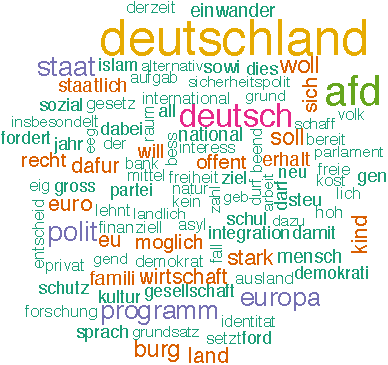
\includegraphics[width=0.7\linewidth]{090_Textmining_files/figure-latex/unnamed-chunk-18-1} \end{center}

Man kann die Anzahl der Wörter, Farben und einige weitere Formatierungen
der Wortwolke beeinflussen\footnote{\url{https://cran.r-project.org/web/packages/wordcloud/index.html}}.

Weniger verspielt ist eine schlichte visualisierte Häufigkeitsauszählung
dieser Art, z.B. mit Balkendiagrammen (gedreht).

\begin{Shaded}
\begin{Highlighting}[]

\NormalTok{afd_count %>%}\StringTok{ }
\StringTok{  }\KeywordTok{top_n}\NormalTok{(}\DecValTok{30}\NormalTok{) %>%}\StringTok{ }
\StringTok{  }\KeywordTok{ggplot}\NormalTok{() +}
\StringTok{  }\KeywordTok{aes}\NormalTok{(}\DataTypeTok{x =} \KeywordTok{reorder}\NormalTok{(token_stem, n), }\DataTypeTok{y =} \NormalTok{n) +}
\StringTok{  }\KeywordTok{geom_col}\NormalTok{() +}\StringTok{ }
\StringTok{  }\KeywordTok{labs}\NormalTok{(}\DataTypeTok{title =} \StringTok{"mit Trunkierung"}\NormalTok{) +}
\StringTok{  }\KeywordTok{coord_flip}\NormalTok{() ->}\StringTok{ }\NormalTok{p1}

\NormalTok{afd_df %>%}\StringTok{ }
\StringTok{  }\KeywordTok{count}\NormalTok{(token, }\DataTypeTok{sort =} \OtherTok{TRUE}\NormalTok{) %>%}\StringTok{ }
\StringTok{  }\KeywordTok{top_n}\NormalTok{(}\DecValTok{30}\NormalTok{) %>%}\StringTok{ }
\StringTok{  }\KeywordTok{ggplot}\NormalTok{() +}
\StringTok{  }\KeywordTok{aes}\NormalTok{(}\DataTypeTok{x =} \KeywordTok{reorder}\NormalTok{(token, n), }\DataTypeTok{y =} \NormalTok{n) +}
\StringTok{  }\KeywordTok{geom_col}\NormalTok{() +}
\StringTok{  }\KeywordTok{labs}\NormalTok{(}\DataTypeTok{title =} \StringTok{"ohne Trunkierung"}\NormalTok{) +}
\StringTok{  }\KeywordTok{coord_flip}\NormalTok{() ->}\StringTok{ }\NormalTok{p2}


\KeywordTok{library}\NormalTok{(gridExtra)}
\KeywordTok{grid.arrange}\NormalTok{(p1, p2, }\DataTypeTok{ncol =} \DecValTok{2}\NormalTok{)}
\end{Highlighting}
\end{Shaded}

\begin{center}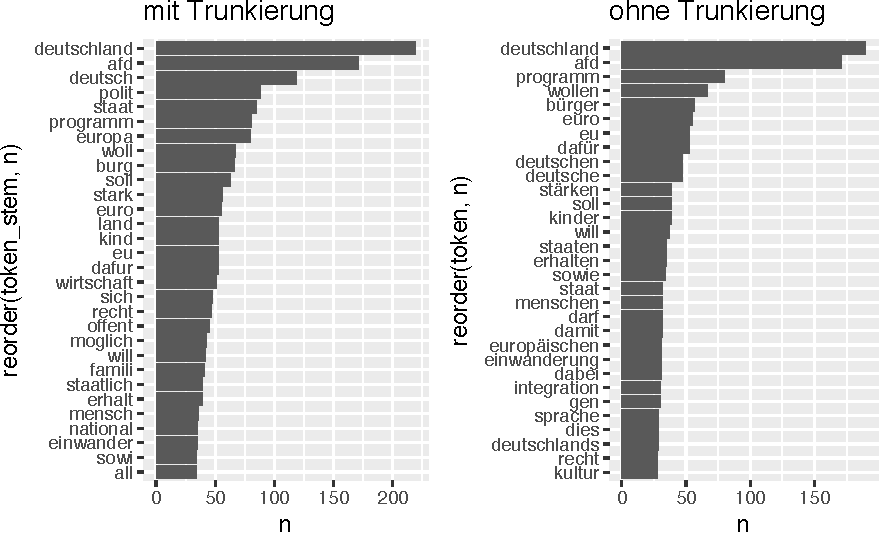
\includegraphics[width=0.7\linewidth]{090_Textmining_files/figure-latex/unnamed-chunk-19-1} \end{center}

Die beiden Diagramme vergleichen die trunkierten Wörter mit den nicht
trunktierten Wörtern. Mit \texttt{reorder} ordnen wir die Spalte
\texttt{token} nach der Spalte \texttt{n}. \texttt{coord\_flip} dreht
die Abbildung um 90°, d.h. die Achsen sind vertauscht.
\texttt{grid.arrange} packt beide Plots in eine Abbildung, welche 2
Spalten (\texttt{ncol}) hat.

\section{Befehlsübersicht}\label{befehlsubersicht}

Tabelle \ref{tab:befehle-text} fasst die R-Funktionen dieses Kapitels
zusammen.

\begin{longtable}[]{@{}ll@{}}
\caption{Befehle des Kapitels `Textmining'}\tabularnewline
\toprule
\begin{minipage}[b]{0.34\columnwidth}\raggedright\strut
Paket..Befehl\strut
\end{minipage} & \begin{minipage}[b]{0.42\columnwidth}\raggedright\strut
Beschreibung\strut
\end{minipage}\tabularnewline
\midrule
\endfirsthead
\toprule
\begin{minipage}[b]{0.34\columnwidth}\raggedright\strut
Paket..Befehl\strut
\end{minipage} & \begin{minipage}[b]{0.42\columnwidth}\raggedright\strut
Beschreibung\strut
\end{minipage}\tabularnewline
\midrule
\endhead
\begin{minipage}[t]{0.34\columnwidth}\raggedright\strut
tidytext::unnest\_tokens\strut
\end{minipage} & \begin{minipage}[t]{0.42\columnwidth}\raggedright\strut
Jedes Token (Wort) einer Spalte bekommt eine eigene Zeile in einem
Dataframe\strut
\end{minipage}\tabularnewline
\begin{minipage}[t]{0.34\columnwidth}\raggedright\strut
stringr::str\_detect\strut
\end{minipage} & \begin{minipage}[t]{0.42\columnwidth}\raggedright\strut
Sucht nach einem String (Text)\strut
\end{minipage}\tabularnewline
\begin{minipage}[t]{0.34\columnwidth}\raggedright\strut
downloader:: download\strut
\end{minipage} & \begin{minipage}[t]{0.42\columnwidth}\raggedright\strut
lädt eine Datei aus dem Internet herunter\strut
\end{minipage}\tabularnewline
\begin{minipage}[t]{0.34\columnwidth}\raggedright\strut
dplyr::rename\strut
\end{minipage} & \begin{minipage}[t]{0.42\columnwidth}\raggedright\strut
Benennt Spalten um\strut
\end{minipage}\tabularnewline
\begin{minipage}[t]{0.34\columnwidth}\raggedright\strut
anti\_join\strut
\end{minipage} & \begin{minipage}[t]{0.42\columnwidth}\raggedright\strut
Führt Dataframes zusammen, so dass nicht matchende Einträge übernommen
werden\strut
\end{minipage}\tabularnewline
\begin{minipage}[t]{0.34\columnwidth}\raggedright\strut
wordcloud::wordcloud\strut
\end{minipage} & \begin{minipage}[t]{0.42\columnwidth}\raggedright\strut
Erstellt eine Wordcloud\strut
\end{minipage}\tabularnewline
\begin{minipage}[t]{0.34\columnwidth}\raggedright\strut
ggplot2::labs\strut
\end{minipage} & \begin{minipage}[t]{0.42\columnwidth}\raggedright\strut
Fügt Titel oder andere Hinweise einem ggplot2-Objekt hinzu\strut
\end{minipage}\tabularnewline
\begin{minipage}[t]{0.34\columnwidth}\raggedright\strut
ggplot2::coord\_flip\strut
\end{minipage} & \begin{minipage}[t]{0.42\columnwidth}\raggedright\strut
Dreht die Achsen um 90 Grad\strut
\end{minipage}\tabularnewline
\bottomrule
\end{longtable}

\section{Verweise}\label{verweise}

\begin{itemize}
\tightlist
\item
  Das Buch \emph{Tidy Text Minig} (Julia und David
  \protect\hyperlink{ref-tidytextminig}{2017}) ist eine hervorragende
  Quelle vertieftem Wissens zum Textmining mit R.
\end{itemize}

\chapter{Placeholder}\label{placeholder-1}

\chapter{Probeklausur}\label{probeklausur}

\chapter{Literaturverzeichnis}\label{literaturverzeichnis}

\hypertarget{refs}{}
\hypertarget{ref-R-rmarkdown}{}
Allaire, JJ, Joe Cheng, Yihui Xie, Jonathan McPherson, Winston Chang,
Jeff Allen, Hadley Wickham, Aron Atkins, und Rob Hyndman. 2016a.
\emph{rmarkdown: Dynamic Documents for R}.
\url{https://CRAN.R-project.org/package=rmarkdown}.

\hypertarget{ref-rmarkdown}{}
---------. 2016b. \emph{rmarkdown: Dynamic Documents for R}.
\url{https://CRAN.R-project.org/package=rmarkdown}.

\hypertarget{ref-R-gridExtra}{}
Auguie, Baptiste. 2016. \emph{gridExtra: Miscellaneous Functions for
„Grid`` Graphics}. \url{https://CRAN.R-project.org/package=gridExtra}.

\hypertarget{ref-R-BaylorEdPsych}{}
Beaujean, A. Alexander. 2012. \emph{BaylorEdPsych: R Package for Baylor
University Educational Psychology Quantitative Courses}.
\url{https://CRAN.R-project.org/package=BaylorEdPsych}.

\hypertarget{ref-R-quanteda}{}
Benoit, Kenneth, und Paul Nulty. 2016. \emph{quanteda: Quantitative
Analysis of Textual Data}.
\url{https://CRAN.R-project.org/package=quanteda}.

\hypertarget{ref-R-SnowballC}{}
Bouchet-Valat, Milan. 2014. \emph{SnowballC: Snowball stemmers based on
the C libstemmer UTF-8 library}.
\url{https://CRAN.R-project.org/package=SnowballC}.

\hypertarget{ref-breaking}{}
Briggs, William M. 2008. \emph{Breaking the Law of Averages: Real-Life
Probability and Statistics in Plain English}. Lulu.com.

\hypertarget{ref-uncertainty}{}
---------. 2016. \emph{Uncertainty: The Soul of Modeling, Probability \&
Statistics}. Springer.

\hypertarget{ref-bryant1995practical}{}
Bryant, PG, und MA Smith. 1995. „Practical Data Analysis: Case Studies
in Business Statistics, Homewood, IL: Richard D``. Irwin Publishing.

\hypertarget{ref-R-downloader}{}
Chang, Winston. 2015. \emph{downloader: Download Files over HTTP and
HTTPS}. \url{https://CRAN.R-project.org/package=downloader}.

\hypertarget{ref-Chapman2015}{}
Chapman, Chris, und Elea McDonnell Feit. 2015. \emph{R for Marketing
Research and Analytics}. New York City: Springer.
doi:\href{https://doi.org/10.1007/978-3-319-14436-8}{10.1007/978-3-319-14436-8}.

\hypertarget{ref-Cleveland}{}
Cleveland, William S. 1993. \emph{Visualizing Data}. Hobart Press.

\hypertarget{ref-cobb2007introductory}{}
Cobb, George W. 2007. „The introductory statistics course: a Ptolemaic
curriculum?`` \emph{Technology Innovations in Statistics Education} 1
(1).

\hypertarget{ref-Cohen1992}{}
Cohen, J. 1992. „A power primer``. \emph{Psychological Bulletin} 112
(1): 155--59.

\hypertarget{ref-cohen_statistical_1988}{}
Cohen, Jacob. 1988. \emph{Statistical Power Analysis for the Behavioral
Sciences}. Routledge. \url{http://dx.doi.org/10.4324/9780203771587}.

\hypertarget{ref-cortez2009modeling}{}
Cortez, Paulo, António Cerdeira, Fernando Almeida, Telmo Matos, und José
Reis. 2009. „Modeling wine preferences by data mining from
physicochemical properties``. \emph{Decision Support Systems} 47 (4).
Elsevier: 547--53.

\hypertarget{ref-R-ggdendro}{}
de Vries, Andrie, und Brian D. Ripley. 2016. \emph{ggdendro: Create
Dendrograms and Tree Diagrams Using 'ggplot2'}.
\url{https://CRAN.R-project.org/package=ggdendro}.

\hypertarget{ref-introstats}{}
Diez, David M, Christopher D Barr, und Mine Cetinkaya-Rundel. 2014.
\emph{Introductory Statistics with Randomization and Simulation}. North
Charleston, South Carolina: CreateSpace Independent Publishing Platform.

\hypertarget{ref-eid2010statistik}{}
Eid, Michael, Mario Gollwitzer, und Manfred Schmitt. 2010.
\emph{Statistik und Forschungsmethoden}. Göttingen: Hogrefe.

\hypertarget{ref-etz2016become}{}
Etz, Alexander, Quentin Frederik Gronau, Fabian Dablander, Peter
Edelsbrunner, und Beth Baribault. 2016. „How to become a Bayesian in
eight easy steps: An annotated reading list``. PsyArXiv.

\hypertarget{ref-R-tm}{}
Feinerer, Ingo, und Kurt Hornik. 2015. \emph{tm: Text Mining Package}.
\url{https://CRAN.R-project.org/package=tm}.

\hypertarget{ref-R-wordcloud}{}
Fellows, Ian. 2014. \emph{wordcloud: Word Clouds}.
\url{https://CRAN.R-project.org/package=wordcloud}.

\hypertarget{ref-fjalnes_orthogonale_2014}{}
Fjalnes. 2014. „Orthogonale Faktorrotation``.
\url{https://de.wikipedia.org/wiki/Rotationsverfahren_(Statistik)\#/media/File:Orthogonale_faktorrotation.svg}.

\hypertarget{ref-R-car}{}
Fox, John, und Sanford Weisberg. 2016. \emph{car: Companion to Applied
Regression}. \url{https://CRAN.R-project.org/package=car}.

\hypertarget{ref-Gansser_2017}{}
Gansser, Oliver. 2017. „Data for Principal Component Analysis and Common
Factor Analysis``. Open Science Framework. \url{osf.io/zg89r}.

\hypertarget{ref-gigerenzer1980}{}
Gigerenzer, Gerd. 1980. \emph{Messung und Modellbildung in der
Psychologie (Uni-Taschenbucher. Psychologie, Padagogik, Soziologie,
Psychiatrie) (German Edition)}. E. Reinhardt.

\hypertarget{ref-Gigerenzer2004}{}
---------. 2004. „Mindless statistics``. \emph{The Journal of
Socio-Economics} 33 (5). Elsevier BV: 587--606.
doi:\href{https://doi.org/10.1016/j.socec.2004.09.033}{10.1016/j.socec.2004.09.033}.

\hypertarget{ref-god_i_2016}{}
God. 2016. „I don't care about you. Please share this with friends.``
Twitter Tweet. \emph{TheTweetOfGod}.
\url{https://twitter.com/TheTweetOfGod/status/688035049187454976}.

\hypertarget{ref-grolemund2014cognitive}{}
Grolemund, Garrett, und Hadley Wickham. 2014. „A cognitive
interpretation of data analysis``. \emph{International Statistical
Review} 82 (2). Wiley Online Library: 184--204.

\hypertarget{ref-R-arules}{}
Hahsler, Michael, Christian Buchta, Bettina Gruen, und Kurt Hornik.
2016. \emph{arules: Mining Association Rules and Frequent Itemsets}.
\url{https://CRAN.R-project.org/package=arules}.

\hypertarget{ref-R-arulesViz}{}
Hahsler, Michael, und Sudheer Chelluboina. 2016. \emph{arulesViz:
Visualizing Association Rules and Frequent Itemsets}.
\url{https://CRAN.R-project.org/package=arulesViz}.

\hypertarget{ref-hamermesh2005beauty}{}
Hamermesh, Daniel S, und Amy Parker. 2005. „Beauty in the classroom:
Instructors' pulchritude and putative pedagogical productivity``.
\emph{Economics of Education Review} 24 (4). Elsevier: 369--76.

\hypertarget{ref-hardin2015data}{}
Hardin, Johanna, Roger Hoerl, Nicholas J Horton, Deborah Nolan, Ben
Baumer, Olaf Hall-Holt, Paul Murrell, u.~a. 2015. „Data science in
statistics curricula: Preparing students to 'Think with Data'``.
\emph{The American Statistician} 69 (4). Taylor \& Francis: 343--53.

\hypertarget{ref-Hatzinger}{}
Hatzinger, Reinhold, Kurt Hornik, und Herbert Nagel. 2014. \emph{R-
Einfuehrung durch angewandte Statistik}. Pearson Studium.

\hypertarget{ref-Head2015}{}
Head, Megan L., Luke Holman, Rob Lanfear, Andrew T. Kahn, und Michael D.
Jennions. 2015. „The Extent and Consequences of P-Hacking in Science``.
\emph{PLOS Biology} 13 (3). Public Library of Science (PLoS): e1002106.
doi:\href{https://doi.org/10.1371/journal.pbio.1002106}{10.1371/journal.pbio.1002106}.

\hypertarget{ref-R-titanic}{}
Hendricks, Paul. 2015. \emph{titanic: Titanic Passenger Survival Data
Set}. \url{https://CRAN.R-project.org/package=titanic}.

\hypertarget{ref-hoekstra2014robust}{}
Hoekstra, Rink, Richard D Morey, Jeffrey N Rouder, und Eric-Jan
Wagenmakers. 2014. „Robust misinterpretation of confidence intervals``.
\emph{Psychonomic bulletin \& review} 21 (5). Springer: 1157--64.

\hypertarget{ref-hyndman2014forecasting}{}
Hyndman, R.J., und G. Athanasopoulos. 2014. \emph{Forecasting:
principles and practice:} OTexts.
\url{https://books.google.de/books?id=gDuRBAAAQBAJ}.

\hypertarget{ref-tm}{}
Ingo Feinerer, Kurt Hornik, und David Meyer. 2008. „Text Mining
Infrastructure in R``. \emph{Journal of Statistical Software} 25 (5):
1--54. \url{http://www.jstatsoft.org/v25/i05/}.

\hypertarget{ref-R-corrr}{}
Jackson, Simon. 2016. \emph{corrr: Correlations in R}.
\url{https://CRAN.R-project.org/package=corrr}.

\hypertarget{ref-R-ISLR}{}
James, Gareth, Daniela Witten, Trevor Hastie, und Rob Tibshirani. 2013a.
\emph{ISLR: Data for An Introduction to Statistical Learning with
Applications in R}. \url{https://CRAN.R-project.org/package=ISLR}.

\hypertarget{ref-introstatlearning}{}
James, Gareth, Daniela Witten, Trevor Hastie, und Robert Tibshirani.
2013b. \emph{An introduction to statistical learning}. Bd. 6. Springer.

\hypertarget{ref-james2013introduction}{}
---------. 2013c. \emph{An introduction to statistical learning}. Bd. 6.
Springer.

\hypertarget{ref-tidytextminig}{}
Julia, PhD Silge, und PhD Robinson David. 2017. \emph{Text Mining with
R: A tidy approach}. O'Reilly Media.

\hypertarget{ref-kim2015okcupid}{}
Kim, Albert Y, und Adriana Escobedo-Land. 2015. „OkCupid Data for
Introductory Statistics and Data Science Courses``. \emph{Journal of
Statistics Education} 23 (2). Citeseer: n2.

\hypertarget{ref-R-okcupiddata}{}
Kim, Albert Y., und Adriana Escobedo-Land. 2016. \emph{okcupiddata:
OkCupid Profile Data for Introductory Statistics and Data Science
Courses}. \url{https://CRAN.R-project.org/package=okcupiddata}.

\hypertarget{ref-kraemer2011wir}{}
Krämer, W. 2011. \emph{Wie wir uns von falschen Theorien täuschen
lassen}. Berlin University Press.
\url{https://books.google.de/books?id=HWUKaAEACAAJ}.

\hypertarget{ref-kruschke2010bayesian}{}
Kruschke, John K. 2010. „Bayesian data analysis``. \emph{Wiley
Interdisciplinary Reviews: Cognitive Science} 1 (5). Burlington, MA:
Academic Press: 658--76.

\hypertarget{ref-kuhn2013applied}{}
Kuhn, Max, und Kjell Johnson. 2013. \emph{Applied predictive modeling}.
Bd. 26. Springer.

\hypertarget{ref-ladyofhats_smileys_2017}{}
LadyOfHats. 2017. „Smileys``.
\url{https://commons.wikimedia.org/wiki/User:LadyofHats\#Smileys}.

\hypertarget{ref-R-scatterplot3d}{}
Ligges, Uwe, Martin Maechler, und Sarah Schnackenberg. 2017.
\emph{scatterplot3d: 3D Scatter Plot}.
\url{https://CRAN.R-project.org/package=scatterplot3d}.

\hypertarget{ref-lubke2014angewandte}{}
Lübke, Karsten, und Martin Vogt. 2014. \emph{Angewandte
Wirtschaftsstatistik: Daten und Zufall}. Berlin: Springer.

\hypertarget{ref-m7_savinellis_2004}{}
M7. 2004. „Savinelli's Italian smoking pipe``.
\url{https://commons.wikimedia.org/wiki/File:Pipa_savinelli.jpg}.

\hypertarget{ref-matejka2017same}{}
Matejka, Justin, und George Fitzmaurice. 2017. „Same stats, different
graphs: Generating datasets with varied appearance and identical
statistics through simulated annealing``. In \emph{Proceedings of the
2017 CHI Conference on Human Factors in Computing Systems}, 1290--4.
ACM.

\hypertarget{ref-R-rpart.plot}{}
Milborrow, Stephen. 2017. \emph{rpart.plot: Plot 'rpart' Models: An
Enhanced Version of 'plot.rpart'}.
\url{https://CRAN.R-project.org/package=rpart.plot}.

\hypertarget{ref-moore1990uncertainty}{}
Moore, David S. 1990. „Uncertainty``. \emph{On the shoulders of giants:
New approaches to numeracy}. ERIC, 95--137.

\hypertarget{ref-R-tokenizers}{}
Mullen, Lincoln. 2016. \emph{tokenizers: A Consistent Interface to
Tokenize Natural Language Text}.
\url{https://CRAN.R-project.org/package=tokenizers}.

\hypertarget{ref-R-RColorBrewer}{}
Neuwirth, Erich. 2014. \emph{RColorBrewer: ColorBrewer Palettes}.
\url{https://CRAN.R-project.org/package=RColorBrewer}.

\hypertarget{ref-R-pdftools}{}
Ooms, Jeroen. 2016. \emph{pdftools: Text Extraction and Rendering of PDF
Documents}. \url{https://CRAN.R-project.org/package=pdftools}.

\hypertarget{ref-peirce1955abduction}{}
Peirce, Charles S. 1955. „Abduction and induction``. \emph{Philosophical
writings of Peirce} 11. New York.

\hypertarget{ref-peng2015art}{}
Peng, Roger D, und Elizabeth Matsui. 2015. „The Art of Data Science``.
\emph{A Guide for Anyone Who Works with Data. Skybrude Consulting} 200:
162.

\hypertarget{ref-R-nFactors}{}
Raiche, Gilles, und David Magis. 2011. \emph{nFactors: Parallel Analysis
and Non Graphical Solutions to the Cattell Scree Test}.
\url{https://CRAN.R-project.org/package=nFactors}.

\hypertarget{ref-R-wesanderson}{}
Ram, Karthik, und Hadley Wickham. 2015. \emph{wesanderson: A Wes
Anderson Palette Generator}.
\url{https://CRAN.R-project.org/package=wesanderson}.

\hypertarget{ref-R-compute.es}{}
Re, AC Del. 2014. \emph{compute.es: Compute Effect Sizes}.
\url{https://CRAN.R-project.org/package=compute.es}.

\hypertarget{ref-remquahey2010}{}
Remus, R., U. Quasthoff, und G. Heyer. 2010. „SentiWS -- a Publicly
Available German-language Resource for Sentiment Analysis``. In
\emph{Proceedings of the 7th International Language Resources and
Evaluation (LREC'10)}, 1168--71.

\hypertarget{ref-R-MASS}{}
Ripley, Brian. 2016. \emph{MASS: Support Functions and Datasets for
Venables and Ripley's MASS}.
\url{https://CRAN.R-project.org/package=MASS}.

\hypertarget{ref-nycflights13}{}
RITA, Bureau of transportation statistics. 2013. „nycflights13``.
\url{http://www.transtats.bts.gov/DL_SelectFields.asp?Table_ID=236}.

\hypertarget{ref-R-gutenbergr}{}
Robinson, David. 2016. \emph{gutenbergr: Download and Process Public
Domain Works from Project Gutenberg}.
\url{https://cran.rstudio.com/package=gutenbergr}.

\hypertarget{ref-R-broom}{}
Robinson, David, Matthieu Gomez, Boris Demeshev, Dieter Menne, Benjamin
Nutter, Luke Johnston, Ben Bolker, Francois Briatte, und Hadley Wickham.
2015. \emph{broom: Convert Statistical Analysis Objects into Tidy Data
Frames}. \url{https://CRAN.R-project.org/package=broom}.

\hypertarget{ref-R-tidytext}{}
Robinson, David, und Julia Silge. 2016. \emph{tidytext: Text Mining
using 'dplyr', 'ggplot2', and Other Tidy Tools}.
\url{https://CRAN.R-project.org/package=tidytext}.

\hypertarget{ref-sep-statistics}{}
Romeijn, Jan-Willem. 2016. „Philosophy of Statistics``. In \emph{The
Stanford Encyclopedia of Philosophy}, herausgegeben von Edward N. Zalta,
Winter 2016.
\url{http://plato.stanford.edu/archives/win2016/entries/statistics/}.

\hypertarget{ref-ruckerinfinity}{}
Rucker, Rudy. 2004. \emph{Infinity and the Mind}. Princeton: Princeton
University Press. \url{https://books.google.de/books?id=MD0UAwAAQBAJ}.

\hypertarget{ref-Sauer_2016}{}
Sauer, Sebastian. 2016. „Extraversion Dataset``. Open Science Framework.
doi:\href{https://doi.org/10.17605/OSF.IO/4KGZH}{10.17605/OSF.IO/4KGZH}.

\hypertarget{ref-Sauer_2017}{}
---------. 2017a. „Dataset 'predictors of performance in stats test'``.
Open Science Framework.
doi:\href{https://doi.org/10.17605/OSF.IO/SJHUY}{10.17605/OSF.IO/SJHUY}.

\hypertarget{ref-Sauer_2017a}{}
---------. 2017b. „Dataset 'Height and shoe size'``. Open Science
Framework.
doi:\href{https://doi.org/10.17605/OSF.IO/JA9DW}{10.17605/OSF.IO/JA9DW}.

\hypertarget{ref-sauer_wolff}{}
Sauer, Sebastian, und Alexander Wolff. 2016. „The effect of a status
symbol on success in online dating: an experimental study (data
paper)``. \emph{The Winnower}, August.
doi:\href{https://doi.org/10.15200/winn.147241.13309}{10.15200/winn.147241.13309}.

\hypertarget{ref-R-GGally}{}
Schloerke, Barret, Jason Crowley, Di Cook, Francois Briatte, Moritz
Marbach, Edwin Thoen, Amos Elberg, und Joseph Larmarange. 2016.
\emph{GGally: Extension to 'ggplot2'}.
\url{https://CRAN.R-project.org/package=GGally}.

\hypertarget{ref-Schmidt2007}{}
Schmidt, Peter, Sebastian Bamberg, Eldad Davidov, Johannes Herrmann, und
Shalom H. Schwartz. 2007. „Die Messung von Werten mit dem Portraits
Value Questionnaire``. \emph{Zeitschrift für Sozialpsychologie} 38 (4).
Hogrefe Publishing Group: 261--75.
doi:\href{https://doi.org/10.1024/0044-3514.38.4.261}{10.1024/0044-3514.38.4.261}.

\hypertarget{ref-R-janeaustenr}{}
Silge, Julia. 2016. \emph{janeaustenr: Jane Austen's Complete Novels}.
\url{https://CRAN.R-project.org/package=janeaustenr}.

\hypertarget{ref-tidytext-archive}{}
Silge, Julia, David Robinson, und Jim Hester. 2016. „tidytext: Text
mining using dplyr, ggplot2, and other tidy tools``.
doi:\href{https://doi.org/10.5281/zenodo.56714}{10.5281/zenodo.56714}.

\hypertarget{ref-Silge2016}{}
Silge, Julia, und David Robinson. 2016. „tidytext: Text Mining and
Analysis Using Tidy Data Principles in R``. \emph{The Journal of Open
Source Software} 1 (3). The Open Journal.
doi:\href{https://doi.org/10.21105/joss.00037}{10.21105/joss.00037}.

\hypertarget{ref-spurzem_vw_2017}{}
Spurzem, Lothar. 2017. „VW 1303 von Wiking in 1:87``.
\url{https://de.wikipedia.org/wiki/Modellautomobil\#/media/File:Wiking-Modell_VW_1303_(um_1975).JPG}.

\hypertarget{ref-suppes1962basic}{}
Suppes, Patrick, und Joseph L Zinnes. 1962. \emph{Basic measurement
theory}. Institute for mathematical studies in the social sciences.

\hypertarget{ref-oxford}{}
\emph{The Oxford Dictionary of Statistical Terms}. 2006. Oxford
University Press.

\hypertarget{ref-R-rpart}{}
Therneau, Terry, Beth Atkinson, und Brian Ripley. 2015. \emph{rpart:
Recursive Partitioning and Regression Trees}.
\url{https://CRAN.R-project.org/package=rpart}.

\hypertarget{ref-1930824149}{}
Tufte, Edward R. 1990. \emph{Envisioning Information}. Graphics Press.

\hypertarget{ref-1930824130}{}
---------. 2001. \emph{The Visual Display of Quantitative Information}.
Graphics Press.

\hypertarget{ref-1930824165}{}
---------. 2006. \emph{Beautiful Evidence}. Graphics Press.

\hypertarget{ref-unrau1}{}
Unrau, Sebastian. 2017. „No Title``.
\url{https://unsplash.com/photos/CoD2Q92UaEg}.

\hypertarget{ref-R-SDMTools}{}
VanDerWal, Jeremy, Lorena Falconi, Stephanie Januchowski, Luke Shoo, und
Collin Storlie. 2014. \emph{SDMTools: Species Distribution Modelling
Tools: Tools for processing data associated with species distribution
modelling exercises}. \url{https://CRAN.R-project.org/package=SDMTools}.

\hypertarget{ref-Wagenmakers2007}{}
Wagenmakers, Eric-Jan. 2007. „A practical solution to the pervasive
problems ofp values``. \emph{Psychonomic Bulletin \& Review} 14 (5).
Springer Nature: 779--804.
doi:\href{https://doi.org/10.3758/bf03194105}{10.3758/bf03194105}.

\hypertarget{ref-R-gplots}{}
Warnes, Gregory R., Ben Bolker, Lodewijk Bonebakker, Robert Gentleman,
Wolfgang Huber Andy Liaw, Thomas Lumley, Martin Maechler, u.~a. 2016.
\emph{gplots: Various R Programming Tools for Plotting Data}.
\url{https://CRAN.R-project.org/package=gplots}.

\hypertarget{ref-R-corrplot}{}
Wei, Taiyun, und Viliam Simko. 2016. \emph{corrplot: Visualization of a
Correlation Matrix}. \url{https://CRAN.R-project.org/package=corrplot}.

\hypertarget{ref-Wicherts2016}{}
Wicherts, Jelte M., Coosje L. S. Veldkamp, Hilde E. M. Augusteijn,
Marjan Bakker, Robbie C. M. van Aert, und Marcel A. L. M. van Assen.
2016. „Degrees of Freedom in Planning, Running, Analyzing, and Reporting
Psychological Studies: A Checklist to Avoid p-Hacking``. \emph{Frontiers
in Psychology} 7 (November). Frontiers Media SA.
doi:\href{https://doi.org/10.3389/fpsyg.2016.01832}{10.3389/fpsyg.2016.01832}.

\hypertarget{ref-R-ggplot2}{}
Wickham, Hadley. 2009. \emph{ggplot2: Elegant Graphics for Data
Analysis}. Springer-Verlag New York. \url{http://ggplot2.org}.

\hypertarget{ref-tidydata}{}
---------. 2014. „Tidy Data``. \emph{Journal of Statistical Software} 59
(1): 1--23.
doi:\href{https://doi.org/10.18637/jss.v059.i10}{10.18637/jss.v059.i10}.

\hypertarget{ref-R-reshape2}{}
---------. 2016a. \emph{reshape2: Flexibly Reshape Data: A Reboot of the
Reshape Package}. \url{https://CRAN.R-project.org/package=reshape2}.

\hypertarget{ref-R-tidyr}{}
---------. 2016b. \emph{tidyr: Easily Tidy Data with `spread()` and
`gather()` Functions}. \url{https://CRAN.R-project.org/package=tidyr}.

\hypertarget{ref-R-nycflights13}{}
---------. 2017a. \emph{nycflights13: Flights that Departed NYC in
2013}. \url{https://CRAN.R-project.org/package=nycflights13}.

\hypertarget{ref-R-stringr}{}
---------. 2017b. \emph{stringr: Simple, Consistent Wrappers for Common
String Operations}. \url{https://CRAN.R-project.org/package=stringr}.

\hypertarget{ref-R-tidyverse}{}
---------. 2017c. \emph{tidyverse: Easily Install and Load 'Tidyverse'
Packages}. \url{https://CRAN.R-project.org/package=tidyverse}.

\hypertarget{ref-R-readr}{}
Wickham, Hadley, Jim Hester, und Romain Francois. 2016a. \emph{readr:
Read Tabular Data}. \url{https://CRAN.R-project.org/package=readr}.

\hypertarget{ref-readr}{}
---------. 2016b. \emph{readr: Read Tabular Data}.
\url{https://CRAN.R-project.org/package=readr}.

\hypertarget{ref-R-dplyr}{}
Wickham, Hadley, und Romain Francois. 2016. \emph{dplyr: A Grammar of
Data Manipulation}. \url{https://CRAN.R-project.org/package=dplyr}.

\hypertarget{ref-r4ds}{}
Wickham, Hadley, und Garrett Grolemund. 2016. \emph{R for Data Science:
Visualize, Model, Transform, Tidy, and Import Data}. O'Reilly Media.

\hypertarget{ref-wiki:groesse}{}
Wikipedia. 2017. „Körpergröße --- Wikipedia, Die freie Enzyklopädie``.
\url{https://de.wikipedia.org/w/index.php?title=K\%C3\%B6rpergr\%C3\%B6\%C3\%9Fe\&oldid=165047921}.

\hypertarget{ref-wild1999statistical}{}
Wild, Chris J, und Maxine Pfannkuch. 1999. „Statistical thinking in
empirical enquiry``. \emph{International Statistical Review} 67 (3).
Wiley Online Library: 223--48.

\hypertarget{ref-R-lsa}{}
Wild, Fridolin. 2015. \emph{lsa: Latent Semantic Analysis}.
\url{https://CRAN.R-project.org/package=lsa}.

\hypertarget{ref-wilkinson2006grammar}{}
Wilkinson, Leland. 2006. \emph{The grammar of graphics}. Springer
Science \& Business Media.

\hypertarget{ref-xie2015}{}
Xie, Yihui. 2015. \emph{Dynamic Documents with R and knitr}. 2nd Aufl.
Boca Raton, Florida: Chapman; Hall/CRC. \url{http://yihui.name/knitr/}.

\hypertarget{ref-R-knitr}{}
---------. 2016. \emph{knitr: A General-Purpose Package for Dynamic
Report Generation in R}. \url{https://CRAN.R-project.org/package=knitr}.

\hypertarget{ref-zumel2014practical}{}
Zumel, Nina, John Mount, und Jim Porzak. 2014. \emph{Practical data
science with R}. Manning.

\printindex

\backmatter


\end{document}
